\documentclass[../main.tex]{subfiles}

\begin{document}
\cleartooddpage[\thispagestyle{empty}]
\phantomsection\addcontentsline{toc}{part}{Appendices}
\originalpart*{Appendices}

% \chapter{Material}
% Here follows a brief description of the material used in this thesis
% \section{Hardware}
% A portable personal computer
% \begin{description}
% \item [Processor] Intel(R) Core(TM) i7-8750H CPU @ 2.20GHz
% \item [Memory] 15GiB System memory
% \end{description}
% \section{OS}
% A GNU/Linux system based on architecture x86\_64 with
% \begin{description}
%     \item[Linux kernel] version 5.4.0-73-generic
%     \item[Ubuntu distribution] version \#82~18.04.1-Ubuntu SMP Fri Apr 16 15:10:02 UTC 2021
% \end{description}

% \section{Programming}
% The programs used in this thesis were developed in MATLAB language.

% They were executed on
% \begin{description}
% \item[MATLAB] version R2019b Update 3 (9.7.0.1261785) 64-bit (glnxa64).
% \end{description}

% All code and resulting data is available in \todo{add github link}.

% The graphs based on the saved data were generated using python scripts, also available.

% The scripts were then executed using
% \begin{description}
% \item[python] version 3.6.9
% \end{description}
% with packages:
% \begin{description}
%     \item[matplotlib] version 3.2.2
%     \item[numpy] version 1.19.0
%     \item[scipy] version 1.3.2
% \end{description}
% \section{Writing}
% This thesis was written using GNU Emacs, typeset using \gls{latex}.

% Diagrams were drawn using \gls{TikZ}.

% Hand drawings were drawn using Xournal++ and Inkscape.

\chapter{Résumé étendu en français}

\section{Contexte et Motivation}\label{sec:cont-et-motiv}

L'évolution de la computation dans les dernières deux décades est indéniable.
Dispositifs avec la même puissance des ordinateurs qui ont possibilité l'humanité à toucher le sol lunaire dans la décade de $1970$ sont aujourd'hui à la distance d'une main.

Cette évolution a proportionné l'utilisation de la commande prédictive~\cite{GarciaEtAl1989}, en anglais
connue comme \mpclong{} ou \mpcshort, en problèmes avec échelles de temps réduites, quelquefois en temps-réel~\cite{BesselmannEtAl2008}, et en utilisant dispositifs plus petits qu'une pièce~\cite{BanguraMahony2014}.

Aussi comme conséquence la \mpc{} est envisagée pour contrôler systèmes dans une myriade d'applications avec l'échelle de villes, comme les réseaux de distribution d'eau~\cite{ZhangEtAl2021}, en anglais
\wdns, et de chaleur~\cite{TaylorEtAl2021}, en anglais \dhns.
Ça présente l'insertion de la \mpc{} dans les systèmes cyber-physiques, en anglais \cps{}, où ordinateurs et machines sont étroitement couplées.

Cependant, pour quelques systèmes de grande échelles, le calcul peut encore être coûteuse, nécessitant de stratégies, comme diviser le calcul en plusieurs dispositfs, à fin de faciliter la computation.
Comme on verra cette stratégie est appelée commande prédictive distribuée, ou \dmpc{}, et cela vient en differents moutures.

Néanmoins, pas trop d'études ont été faites pour la sécurité des stratégies \dmpc{}, quand les agents ne communiquent honnêtement.
Ce travail étudie ce que se passe quand les unités ne travaillent pas ensemble.

Pour illustrer on donne un example d'un réseau \dhn{} avec 4 maisons (Fig.~\ref{fig:houses_resume}) qui n'a pas assez de puissance pour répondre aux nécessités de ses résidents, nécessitant d'un compromis.
\begin{figure}[H]
  \centering
  \begin{tikzpicture}[node distance=.5cm and .75cm,scale=1]
    \node[color=mpc_agent] (house1) at (0,0) {\scalebox{2.5}{\faHome}};
    \node[minimum height=1cm,below=of house1] (medium) {};
    \node[color=mpc_agent,right=of medium] (house2)  {\scalebox{3.5}{\faHome}};
    \node[color=mpc_agent,below=of medium] (house3)  {\scalebox{3}{\faHome}};
    \node[color=mpc_agent,left= of medium] (house4)  {\scalebox{4}{\faHome}};

    \draw[latex-,line width=1pt] (house1) -- (medium.center);
    \draw[latex-,line width=1pt] (house2) -- (medium.center);
    \draw[latex-,line width=1pt] (house3) -- (medium.center);
    \draw[latex-,line width=1pt] (house4) -- (medium.center);
    % \draw[latex-,line width=1pt] (house4) -- (medium.center) node[above,midway] {\large $\vec{u}_{i}(t)$};
    \draw[color=black,fill=mpc_coordinator,] (medium) circle [radius=.2cm];

    % \node[latex-,line width=7pt] at ($(house4) +(-1,1)$) {\large $w_{i}(t)$};
    % \node[latex-,line width=7pt] at ($(house4)$) {$\vec{x}_{i}(t)$};

  \end{tikzpicture}
  \caption{\dhn{} avec $4$ maisons.}\label{fig:houses_resume}
\end{figure}

La commande est faite utilisant \mpc{} décomposée avec un coordinateur e un agent local pour chaque maison. On voit le schéma de communication entre les entités dans la Fig.~\ref{fig:echange_controleurs_coordinateur}.
\begin{figure}[h]
  \centering
  \begin{tikzpicture}[font=\small,thick,node distance=3*0.6180cm and 0.6180cm,every node/.style=rectangle,
    mpcSmall/.style={fill=mpc_agent, minimum height=0.6180*2cm, minimum width=2cm},
    coordinator/.style={fill=mpc_coordinator, minimum height=0.6180*3cm, minimum width=6cm},
    ]

    \node[draw, mpcSmall,] (block1) {\small Maison 1};
    \node[fill=none, draw=none, right=of block1,] (mult) {\bf $\dots$};
    \node[draw, mpcSmall, fill=mpc_agent, right=of mult,] (blockM) {\small Maison M};
    \node[draw, coordinator, below=of mult,] (coordinator) {Coordinateur};

    \draw[-latex,line width=1pt] (block1.south)+(0.4,.0) -- ( coordinator.north -| {$(block1.south)+(0.4,.0)$}) node [right,midway] {$\lambdai[1]$};
    \draw[latex-,line width=1pt] (block1.south)+(-0.4,0) -- (  coordinator.north -| {$(block1.south)+(-0.4,0)$}) node [left,midway] {$\thetai[1]$};
    \draw[-latex,line width=1pt] (blockM.south)+(0.4,.0) -- ( coordinator.north -| {$(blockM.south)+(0.4,.0)$}) node [right,midway] {$\lambdai[M]$};
    \draw[latex-,line width=1pt] (blockM.south)+(-0.4,0) -- (  coordinator.north -| {$(blockM.south)+(-0.4,0)$}) node [left,midway] {$\thetai[M]$};
  \end{tikzpicture}
  \caption{Échange entre contrôleurs locaux et coordinateur.}\label{fig:echange_controleurs_coordinateur}
\end{figure}
Les allocations de resources $\thetai$ sont proposées pour chaque maison par le coordinateur.
Le contrôleurs locaux respondent avec des indices $\lambdai$ qui indiquent leur satisfaction.
Les allocations sont mises à jour basées sur ces indices jusq'un consensus soit établi.

Dans un certain moment, un des agents, plus spécifiquement celui correspondant à la maison I, commence a modifier la valeur de $\lambdai$ envoyée.
Il l'augmente a chaque jour jusqu'à un jour la commande est arretée due à une manque de consensus entre les agents.

En utilisant des métriques comme les fonctions objectives, dans laquelle valeures plus petites signifiquent une meilleure perfomance, on peut voir que la performance de l'agent I a amélioré à partir d'une certaine date à la fin d'octobre (Fig.~\ref{fig:change_in_j_resume}).
Par contre, la performance de toutes les autres agents a empiré.
On peut voir aussi dans l'aire hachuré quand le consensus n'est plut trouvé.
\begin{figure}[h]
  \centering
  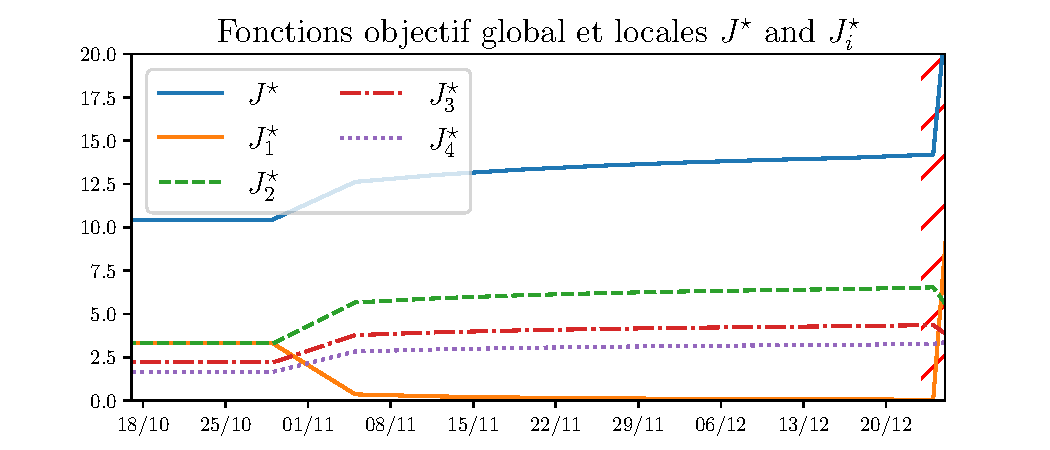
\includegraphics[width=.8\textwidth]{../img/example_introduction/example_J_fr.pdf}
  \caption{Graphique des fonctions objectives dans une période de 10 semaines.}\label{fig:change_in_j_resume}
\end{figure}

Cet example simple nous donne les effets d'un attaque: perte de performance et cassure du fonctionnement du système.
Le même peut arriver causé par des fautes.
Motivé par examples réels comme les black-out de 2010 au Brési~\cite{Conti2010}, l'attaque Stuxnet au Iran en 2011~\cite{Langner2011}, et les attaques à une central électrique en Ukraine in 2016~\cite{Bindra2017} et mal-heusement beaucoup d'autres~\cite{DingEtAl2018,DibajiEtAl2019}, on veut étudier la sécurité des \cps{}.

Dans ce travail on va focaliser sur la securité des \cps{} command par \dmpc{}.

Utilisant la connaisance acquise on propose des méthodes pour sécurises ses systèmes.

On utilise comme guide les questions suivantes:
\simplebox{
  \begin{itemize} \bfseries
    \item Peut-on detecter l'attaque?
    \item Peut-on identifier l'attaqueur?
    \item Peut-ont miniser les effets du dit attaque?
  \end{itemize}
}
Cette thèse a comme objectif répondre ces questions dans un cas spécifique qui sera formalement presenté.
Pour mieux comprendre et répondre ces questions, on divise ce travail en deux parties:

\paragraph{La première partie} (\S\ref{sec:comm-pred-et} à~\ref{sec:comp-anorm}) sert comme une gentille introduction au déssin des \dmpc{}, à sa sécurité et à des attaques.
\newcommand{\tpc}{\textperiodcentered}

Pour un\tpc{}e lecteur\tpc{}ice pas familiarisé\tpc{}e, Section~\ref{sec:comm-pred-et} explique ce qui est une Commande Prédictive et les défis pour la décomposer.
Section~\ref{sec:differents-topologies} discute les topologies possibles pour fair la décomposition.
Section~\ref{sec:comp-anorm} définit comportements anormaux, donne quelques examples, les catégorise et présente les méthodes pour les prévenir et combattre.

\paragraph{La seconde partie} (\S\ref{sec:vulnerabilites-de-la} à~\ref{sec:comm-pred-resil-1}) contient les contributions de cette thèse.

Section~\ref{sec:vulnerabilites-de-la} présente la décomposition étudié (décomposition primal). On presents ses vulnérabilités et comment elles peuvent affecter la perfomance du système.
On formalise l'example en donnant une approche plus quantitative.
Une fois les vulnérabilités et les possibles effets des attaques découverts, on divise la mitigation en parties plus gérable.
\\ Premièrement en Section~\ref{sec:comm-pred-resil}, on analyse un problème simple, pour qu'on puisse apprécier les possibles difficultés qui peuvent être rencontrées pendant le problème de mitigation.
À partir de cette analyse, on propose des mécanismes de detection et mitigation, suivis par un example académique pour illustrer leur fonctionnement.
\\Après, en Section~\ref{sec:comm-pred-resil-1}, on analyse un problème similaire mais avec un coup de théâtre. Comme on verra, une petite modification du problème inital cause une augmentation exponentiel de sa complexité.
L'analyse de ce nouvel problème résulte une stratégie similaire, mais avec modifications adéquates pour renfermer la nature exponentiel du problème.

Finallement, on conclue le travail avec Section~\ref{sec:conclusion_resume}, où on discute les résultats de l'étude, ses bénéfices et inconvénients.
La discussion ouvre des questions qui peuvent inciter des nouveau travaux.
\subsection{Contributions}
Comme un contribution mineure, on démontre l'étude de la vulnérabilité des \dmpc{} basées sur la décomposition primal, qu'au meilleur de nos connaissance n'a pas jamais été étudié.

Comme contributions majeures, deux stratégies de mitigation pour types différents de système de complexité croissante.

La première pour des systèmes lesquels les resources ne sont pas suffisants pour répondre aux nécessités des agents locaux, on les appelle \textbf{Systèmes Dépourvus}.

La seconde, pour une classe des systèmes exponentielment plus complexes, où on assume que les demandes locales respect au moins quelques contraintes. On utilise tel hypothèse pour acquérir des informations en utilisant une méthode qu'on appelle \textbf{pénurie artificielle}.

\subsection{Publications}
Les discussion dans cette thèse a donné comme résultats les publications suivantes:
\begin{itemize}
  \item Publiés
        \begin{description}
          \item[\cite{NogueiraEtAl2021}] Conference article for the SysTol'21
          \item[\cite{NogueiraEtAl2022}] Conference article for the NecSys'22
        \end{description}
\end{itemize}

\newpage
\section{Commande Prédictive et sa décomposition}\label{sec:comm-pred-et}


La commande prédictive basée en modèle, ou commande prédictive, ou encore \mpclong{} en anglais, est une stratégie de commande en boucle fermée basée dans la solution des problèmes d'optimisation.
Ayant un modèle du système à commander et une fonction objective, la stratégie utilise le modèle pour prévoir l'évolution de ses états et computer une séquence optimale de command qui optimise la fonction donnée.
Comme on utilise des problèmes d'optimisation, il est naturel d'ajouter des restriction en forme de contraintes d'égalité et d'inégalité.

Cette stratégie a une place spéciale dans l'industrie et est présente dans une plethora d'applications (gestion d'énérgie~\cite{AnandutaEtAl2018}, commande des quadrotors~\cite{BanguraMahony2014} et autres).

On focalise sur la \mpc{} pour des systèmes linéaires.
\subsection{\mpc{} for linear systems}
The \mpc\ community favors the use of convex problems when possible. Two families of convex problems broadly used are \qp\ and \lp.
In this work, we concentrate on \qp{} problems, which have quadratic objective functions and affine or linear constraints.
Numerous mathematical solvers are apt to solve this kind of problem directly or through equivalent problems.
We can cite non-extensively some solvers such as MATLAB internal QP solvers\footnote{\url{https://fr.mathworks.com/help/optim/ug/quadprog.html}}, OSQP\footnote{\url{https://osqp.org}}, MOSEK\footnote{\url{https://www.mosek.com}} and ECOS\footnote{\url{https://github.com/embotech/ecos}}.

\newpage
\section{Differents topologies}\label{sec:differents-topologies}

\newpage
\section{Comportements anormaux}\label{sec:comp-anorm}

\newpage
\section{Vulnerabilités de la decomposition primal}\label{sec:vulnerabilites-de-la}

\newpage
\section{Commande Prédictive résiliente pour systèmes dépourvus}\label{sec:comm-pred-resil}
\newpage
\section{Commande Prédictive résiliente sur pénurie artificielle}\label{sec:comm-pred-resil-1}

\newpage
\section{Conclusion}\label{sec:conclusion_resume}
\end{document}
